%% Basierend auf einer TeXnicCenter-Vorlage von Tino Weinkauf.
%%%%%%%%%%%%%%%%%%%%%%%%%%%%%%%%%%%%%%%%%%%%%%%%%%%%%%%%%%%%%%

%%%%%%%%%%%%%%%%%%%%%%%%%%%%%%%%%%%%%%%%%%%%%%%%%%%%%%%%%%%%%
%% HEADER
%%%%%%%%%%%%%%%%%%%%%%%%%%%%%%%%%%%%%%%%%%%%%%%%%%%%%%%%%%%%%
\documentclass[a4paper,oneside,12pt]{article}
\usepackage{geometry}
\geometry{a4paper,left=40mm,right=30mm, top=25mm, bottom=25mm} 
% Alternative Optionen:
%	Papiergr��e: a4paper / a5paper / b5paper / letterpaper / legalpaper / executivepaper
% Duplex: oneside / twoside
% Grundlegende Fontgr��en: 10pt / 11pt / 12pt


%% Deutsche Anpassungen %%%%%%%%%%%%%%%%%%%%%%%%%%%%%%%%%%%%%
\usepackage[ngerman]{babel}
\usepackage[utf8]{inputenc}
\usepackage[T1]{fontenc}
\usepackage{lmodern} %Type1-Schriftart f�r nicht-englische Texte
\usepackage{float}
\usepackage{floatflt}

%% Packages f�r Grafiken & Abbildungen %%%%%%%%%%%%%%%%%%%%%%
\usepackage{graphicx} %%Zum Laden von Grafiken
%\usepackage{subfig} %%Teilabbildungen in einer Abbildung
%\usepackage{pst-all} %%PSTricks - nicht verwendbar mit pdfLaTeX

%% Beachten Sie:
%% Die Einbindung einer Grafik erfolgt mit \includegraphics{Dateiname}
%% bzw. �ber den Dialog im Einf�gen-Men�.
%% 
%% Im Modus "LaTeX => PDF" k�nnen Sie u.a. folgende Grafikformate verwenden:
%%   .jpg  .png  .pdf  .mps
%% 
%% In den Modi "LaTeX => DVI", "LaTeX => PS" und "LaTeX => PS => PDF"
%% k�nnen Sie u.a. folgende Grafikformate verwenden:
%%   .eps  .ps  .bmp  .pict  .pntg


%% Packages f�r Formeln %%%%%%%%%%%%%%%%%%%%%%%%%%%%%%%%%%%%%
\usepackage{amsmath}
\usepackage{amsthm}
\usepackage{amsfonts}


%% Zeilenabstand %%%%%%%%%%%%%%%%%%%%%%%%%%%%%%%%%%%%%%%%%%%%
%\usepackage{setspace}
%\singlespacing        %% 1-zeilig (Standard)
%\onehalfspacing       %% 1,5-zeilig
%\doublespacing        %% 2-zeilig


%% Farben %%%%%%%%%%%%%%%%%%%%%%%%%%%%%%%%%%%%%%%%%%%%%%%%%%%
\usepackage{color}
\usepackage{framed}
\usepackage{colortbl}
\definecolor{middlegray}{rgb}{0.5,0.5,0.5}
\definecolor{lightgray}{rgb}{0.8,0.8,0.8}
\definecolor{orange}{rgb}{0.8,0.3,0.3}
\definecolor{yac}{rgb}{0.6,0.6,0.1}
\definecolor{darkgray}{rgb}{0.3,0.3,0.3}
\definecolor{blue}{rgb}{0,0,1}
\definecolor{green}{rgb}{0,0.6,0}
\definecolor{yellow}{rgb}{1,1,0}
\definecolor{shadecolor}{gray}{.85}
\usepackage[table]{xcolor}
\newcommand{\tblue}{\cellcolor{blue!25}}
\newcommand{\tred}{\cellcolor{red!25}}
\newcommand{\tgreen}{\cellcolor{green!25}}
\newcommand{\tyellow}{\cellcolor{yellow!25}}


%% CodeListings %%%%%%%%%%%%%%%%%%%%%%%%%%%%%%%%%%%%%%%%%%%%%
\usepackage{listings}
\lstset{
	basicstyle=\scriptsize\ttfamily,
	keywordstyle=\bfseries\ttfamily\color{blue},
	breaklines=true,
	stringstyle=\color{darkgray}\ttfamily,
	commentstyle=\color{green}\ttfamily,
	emph={square}, 
	emphstyle=\color{blue}\texttt,
	emph={[2]root,base},
	emphstyle={[2]\color{yac}\texttt},
	showstringspaces=false,
	flexiblecolumns=false,
	captionpos=b,
	tabsize=2,
	numbers=left,
	numberstyle=\tiny,
	numberblanklines=true,
	stepnumber=1,
	numbersep=10pt,
	xleftmargin=15pt,
	frame=single
}

%% Verlinktes Inhaltsverzeichnis %%%%%%%%%%%%%%%%%%%%%%%%%%%
\usepackage[colorlinks,
pdfpagelabels,
pdfstartview = FitH,
bookmarksopen = true,
bookmarksnumbered = true,
linkcolor = black,
plainpages = false,
hypertexnames = false,
citecolor = black] {hyperref}


%% Sonstiges %%%%%%%%%%%%%%%%%%%%%%%%%%%%%%%%%%%%%%%%%%%%%%%
\usepackage{float}
\usepackage{tabularx}
\usepackage{amsmath}
\usepackage{subfigure}
\usepackage{multirow}
\usepackage{ulem}
\usepackage{wrapfig}

\setlength{\parindent}{0pt}


%% Andere Packages %%%%%%%%%%%%%%%%%%%%%%%%%%%%%%%%%%%%%%%%%%
%\usepackage{a4wide} %%Kleinere Seitenr�nder = mehr Text pro Zeile.
%\usepackage{fancyhdr} %%Fancy Kopf- und Fu�zeilen
%\usepackage{longtable} %%F�r Tabellen, die eine Seite �berschreiten


%% execute scripts %%%%%%%%%%%%%%%%%%%%%%%%%%%%%%%%%%%%%%%%%%
\newcommand{\visioToPDF}[1] {
	\immediate\write18{convert_scripts\string\\visioToPDF.bat #1}
}


%%%%%%%%%%%%%%%%%%%%%%%%%%%%%%%%%%%%%%%%%%%%%%%%%%%%%%%%%%%%%
%% Anmerkungen
%%%%%%%%%%%%%%%%%%%%%%%%%%%%%%%%%%%%%%%%%%%%%%%%%%%%%%%%%%%%%
%
% Zu erledigen:
% 1. Passen Sie die Packages und deren Optionen an (siehe oben).
% 2. Wenn Sie wollen, erstellen Sie eine BibTeX-Datei
%    (z.B. 'literatur.bib').
% 3. Happy TeXing!
%
%%%%%%%%%%%%%%%%%%%%%%%%%%%%%%%%%%%%%%%%%%%%%%%%%%%%%%%%%%%%%


%%%%%%%%%%%%%%%%%%%%%%%%%%%%%%%%%%%%%%%%%%%%%%%%%%%%%%%%%%%%%
%% Optionen / Modifikationen
%%%%%%%%%%%%%%%%%%%%%%%%%%%%%%%%%%%%%%%%%%%%%%%%%%%%%%%%%%%%%

%\input{optionen} %Eine Datei 'optionen.tex' wird hierf�r ben�tigt.
%% ==> TeXnicCenter liefert m�gliche Optionendateien
%% ==> im Vorlagenarchiv mit (Datei | Neu von Vorlage...).


%%%%%%%%%%%%%%%%%%%%%%%%%%%%%%%%%%%%%%%%%%%%%%%%%%%%%%%%%%%%%
%% DOKUMENT
%%%%%%%%%%%%%%%%%%%%%%%%%%%%%%%%%%%%%%%%%%%%%%%%%%%%%%%%%%%%%
\begin{document}
\thispagestyle{empty}

\title {
	\huge \textsc{HeartRate2Go}
}
	
\author {
	\begin{tabular}{rl}
		\large Matthias Böffel & \small Matrikel Nr.: 864483 \\ 
		\large Patrick Mathias & \small Matrikel Nr.: 864089 \\ 
		\large Markus Nebel & \small Matrikel Nr.: 864681 \\ 
		\large Janina Sauer & \small Matrikel Nr.: 865235 \\ 
	\end{tabular}
}

\maketitle
\vfill
\begin{figure}[H]
\centering
\small Hochschule Kaiserslautern\\University of Applied Sciences\\
\bigskip
\large Betreuer: Prof. Dr.-Ing. Jan Conrad\\
\bigskip

\includegraphics[scale=0.4]{images/hskllogo.jpg}  
\end{figure}

\newpage
\tableofcontents
%\cleardoublepage %Das erste Kapitel soll auf einer ungeraden Seite beginnen.
%\pagestyle{plain} %%Ab hier die Kopf-/Fusszeilen: headings / fancy / ...

%TODOs: 
%
%In der Abgabe sollen die folgenden Elemente enthalten sein:
%1. Kommentierte Quelltexte und alle Dateien, die für das Bauen und Ausführen der Anwendung 		benötigt werden
%2. Eine ausführbare Version Ihrer Anwendung mit einer Beschreibung z.B. als liesmich.txt die darlegt, wie die Anwendung installiert und ausgeführt wird.
%3. Eine Dokumentation des Projekts im PDF-Format, nähere Infos hierzu finden Sie weiter unten
%
%
%
%Die Dokumentation soll mindestens die folgenden Punkte behandeln:
%1. Beschreibung der von Ihnen implementierten Anwendungen und ihrer Funktionalitäten auf Basis des Konzeptpapiers
%2. Welches Framework haben Sie verwendet? Begründen Sie Ihre Auswahl (macht Patrick)
%3. Beschreibung des Software-Designs
%4. Beschreibung des von Ihnen erstellten User Interface
%5. Eine kurze Beschreibung der Bedienung Ihrer Anwendung
%6. Weitere Angaben zu Ihrem Projekt, falls Sie dies für sinnvoll halten
%7. Verwendete Literatur und Quellen
%8. Retrospektive: Kritischer Rückblick und Vergleich der ursprüngliche Planung mit den
%erzielten Ergebnissen (macht Patrick)
%10. Die von allen Projektmitgliedern unterschriebene „Ausgabe der Projektarbeit und
%Nutzungsvereinbarung“ und „Ehrenwörtliche Erklärung“. Die zwei zu verwendenden
%Vordrucke befinden sich am Ende dieses Dokumentes. (Bös Unterschrift fehlt noch)


\newpage
\section{Einleitung} \label{sec:Einleitung}
\subsection{Vorstellung des Projektes} \label{sec:Vorstellung des Projektes}
Im Projekt \textit{HeartRate2Go} geht es darum, mit einer App für eine Android Uhr die Herzfrequenz per Pulsoxymetrie zu messen und diese Messwerte in einer passenden GUI darzustellen. \\
Somit soll der Anwender bei der Kontrolle seines Pulses unterstützt werden und ihm einen guten, verständlichen Überblick bieten. Dies gilt sowohl für eine Ruhemessung, als auch für eine Messung während einer Aktivität. \\
\\
%Ablauf einer Messung, vllt mit Diagramm 
%Anwender trägt Uhr, startet App, wählt Messart aus, Messung startet, evtl Messung beenden, Abfrage über Stimmung, Smartphone zeigt Durchschnittswert an, Smartphone empfängt Daten automatisch von der Uhr, Smartphone zeigt Werte im Balkendiagramm an, GUI öffnen, GUI empfängt Messdaten per tcp über Smartphone (wird vom Smartphone gesteuert), Messdaten werden in GUI eingefügt und graphisch dargestellt, Messwerte können mit vergangen Messungen verglichen und auch gedruckt werden.
\textbf{Ablauf}\\
\\
Für die Nutzung für \textit{HeartRate2Go} sind drei Komponenten nötig:\\
\begin{itemize}
	\item Android-Uhr
	\item Android-Smartphone und
	\item Computer
\end{itemize}

Der Nutzer trägt die Android-Uhr am Handgelenk und startet auf dieser die \textit{HeartRate2Go-App}. Hier wird nun abgefragt, ob er eine Ruhemessung oder eine Aktivitätsmessung durchführen möchte. Anschließend wird die ausgewählte Messung durchgeführt. Bei einer Ruhemessung wird die Messung automatisch beendet, bei der Aktivitätsmessung muss der Benutzer die Messung manuell beenden. 
Nun wird der Anwender nach seiner Stimmung während der Pulsmessung gefragt, hier hat er die Auswahl zwischen gut, ok und schlecht. Außerdem wird der Durchschnittswert der soeben durchgeführten Messung gezeigt.\\
Die Übertragung der Messwerte von der Android-Uhr an das Android-Smartphone verläuft automatisch per Bluetooth. Auf der Smartphone-App werden die Messungen in einem Balkendiagramm angezeigt und bieten so einen ersten Überblick. \\
\\
\begin{figure} [H]
	\centering
		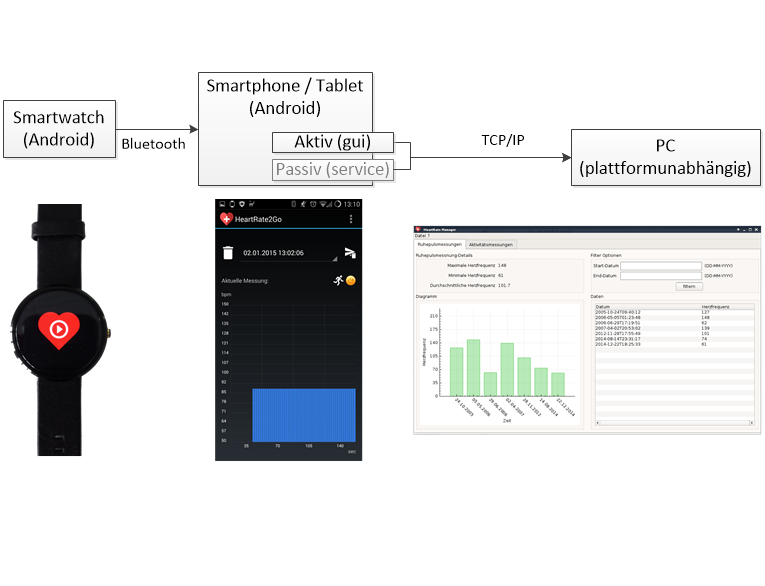
\includegraphics[scale=0.5]{images/ablauf.png}
		\caption{Ablaufdiagramm}
	\label{fig:ablauf}
\end{figure}

\subsection{Medizinische Apps}\label{sec:Medizinische Apps}
Im Laufe der letzten Jahre wurde der Markt mit Apps, die einen medizinischen Hintergrund besitzen, überschüttet. Wenn man im deutschen iTunes-Store nach „Medizin“ sucht, erhält man mehrere hundert Einträge, dies gilt genauso für den Google-Play Store. \\
Im vergangen Jahr sind die Absatzzahlen von medizinischen Apps in Großbritannien, Frankreich, Niederlande und Deutschland um 42 Prozent gestiegen, vermeldet das GfK (Marktforschungszentrum).\\
Diese Apps decken nahezu jeden Bereich der Medizin ab, egal ob es um die Speicherung von Vitaldaten, die Messung von Vitaldaten mit einem zusätzlichen Messgerät und die Auswertung der Daten geht. Des Weiteren sind auch viele Nachschlagewerke darunter enthalten.\\
Zu beachten ist allerdings, dass keiner der Apps den Arztbesuch ersetzt. Sie geben lediglich eine erste Einschätzung und sind dadurch eine große Erleichterung für den Nutzer. Allerdings ist es auch so, dass jeder Programmierer eine App mit medizinischem Hintergrund in die verschiedenen Stores hochladen darf. Diese werde nicht auf ihren Nutzen hin überprüft, so sind auch viele Apps zu finden, die mehr als Spielerei gelten.\\
Kaum eine App ist ein Medizinprodukt nach dem Medizinproduktegesetzt, sie gelten lediglich als Wellness- beziehungsweise Lifestyle-Apps. \\
\\

\textbf{} 
%Thema und Zielsetzung: Stellen Sie zunächst Thema und Zielstellung der Arbeit vor.
%Theorie: Vermitteln Sie Ihre Theorie(n) über das Thema und geben Sie an, auf was sich Ihre Theorie stützt.
%Fragestellung: Teilen Sie mit, welche Fragen in der folgenden Arbeit beantwortet werden.
%Quellen: Welche Quellen haben Sie für Ihre Arbeit genutzt bzw. wie haben Sie Ihre Frage(n) beantwortet?
%Ergebnis: Führen Sie Ihre Ergebnisse auf, also teilen Sie mit, was Sie herausgefunden haben.
%Fazit: Stellen Sie am Ende des Abstracts eine Quintessenz auf. Sie können Ihr Fazit auch mit einer %Zukunftsprognose verbinden.

\subsection{Medizinische Kenntnisse - Pulsoxymetrie} 
Für die Messung des peripheren Pulses per Android-Uhr wird das Prinzip der Reflexions-Pulsoxymetrie genutzt (Abbildung \ref{pic:pulsoxy}).\\
Dieses Verfahren benötigt zwei Sensoren: zum einen eine Lichtquelle, zum anderen ein Lichtsensor. Die Lichtquelle sendet Infrarot-Lichtwellen aus, die durch die Haut dringen. Der Sensor misst die Lichtanteile, die absorbiert wurden. \\
Die Lichtabsorption im Blut ist abhänig von der Hämoglobinkonzentration und der Sättigung des Hämoglobins mit Sauerstoff. Oxigeniertes und desoxigeniertes Hämoglobin schwächen das Licht jeweils charakteristisch ab. \\
Mit diesem Prinzip ist es auch möglich, die Sauerstoffsättigung im kapillären Blut gemessen werden\cite{behandlungsassitenz}.
\begin{figure}[H]
	\centering
	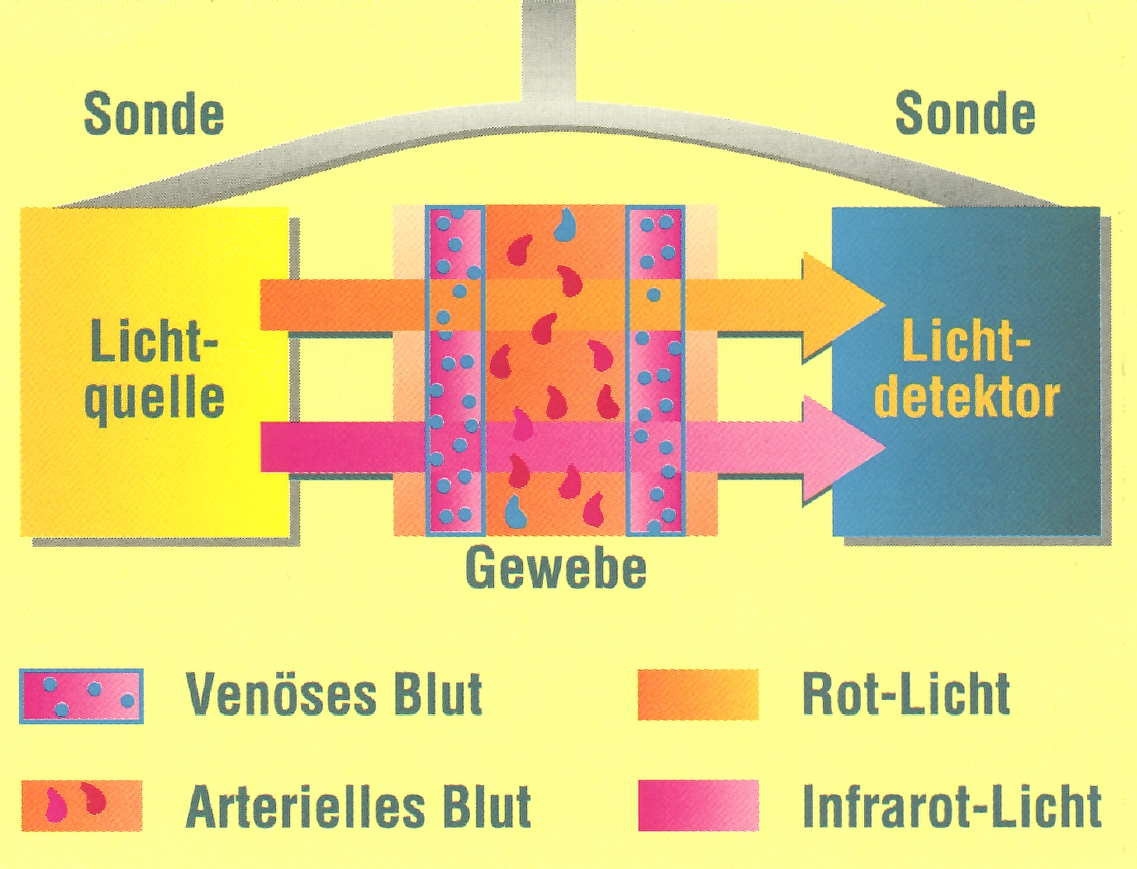
\includegraphics[scale=1.0]{images/pulsoxy.jpg}
	\caption{Veranschaulichung der Pulsoxymetrie\cite{messprinzip-pulsoxi}}
	\label{pic:pulsoxy}
\end{figure}

% Kurze Erklärung 
% reicht das oder noch mehr?
TODO:
bitte Korrektur lesen
Quelle einfügen
Quelle: Behandlungsassistenz „… in der Arztpraxis“ von Dr. Uta Groger, Cornelsen Verlag, 1. Auflage, 2007




\newpage
\section{Wearable \& Handheld} \label{sec:hauptteil_android}

\subsection{Android (Standard)}
Das Android-Betriebsystem erfreut sich weltweit größter Beliebtheit. Android ist mit über 75\% auf dem Markt das meist verbreitete Mobil-Betriebssystem für Smartphones und Tablets. Ein großer Vorteil des mobilen Betriebssystems ist die Möglichkeit, die Funktionalität durch Installation zusätzlicher Anwendungen (Apps) zu erweitern.
\\[0.5cm]
Erstellt werden Apps i.d.R. mit Hilfe des Android-Frameworks in der Programmiersprache Java. Das Android-Framework passt in die Kategorie der modernen GUI-Frameworks, da die Programmlogik strikt von den Definitionen für das Layout getrennt ist. Das Layout wird durch Dateien mit XML-Struktur festgelegt und kann so unabhängig vom Code angepasst werden.

\subsection{Android Wear}
Android Wear als noch recht neues Betriebssystem stellt eine ressourcenschonende Version des Standard-Android-Betriebssystems für Wearables (Smartwatches, Armbänder, etc.) dar. Die Wearables bringen in den meisten Fällen Sensoren für Fitness-Tracking (z.B. Pulsmesser, und Schrittzähler) mit, die durch die Android-API bereits unterstützt werden. Das Wearable-Gerät kann zwar selbstständig agieren, ist jedoch ohne entsprechende Hardware zur Nutzung von Internet, W-LAN oder anderen Ressourcen auf ein gekoppeltes Handheld-Gerät angewiesen. Auch Hersteller Google betont, dass das Betriebssystem grundlegend zur Kopplung mit einem Smartphone bzw. Tablet (im Folgenden allgemein: Handheld) ausgelegt ist. Notifications vom Handheld werden beispielsweise bequem auf das Wearable-Gerät weitergeleitet, während in die andere Richtung Spracheingaben auf dem Wearable-Gerät interpretiert und zum Handheld-Gerät zur weiteren Verarbeitung übermittelt werden können. Die Kommunikation findet dabei i.d.R. über eine spezielle Wearable-Bluetooth-API statt.
\\[0.5cm]
Die Design-Prinzipien, die grundlegend auf den Entwicklerseiten von Android Wear\cite{android-wear-dev} empfohlen werden, unterstreichen ebenfalls die enge Verbundenheit zum Handheld-Gerät. So sollen rechen- bzw. zeitintensive Tasks auf das leistungsfähigere Handheld-Gerät ausgelagert werden und Konfigurationen für Wearable-Apps weitestgehend auf dem Handheld-Gerät vorgenommen werden. So bietet es sich an für eine Wearable-App gleich eine zugehörige Handheld-App mitzuliefern. Die Installation einer Wearable-App erfolgt dabei auch über das Handheld-Gerät: Eine APK-Installations-Datei kann mehrere Apps für verschiedene Geräte enthalten, die dann automatisch verteilt werden. Apps für Android Wear werden unter den gleichen Bedingungen erstellt wie Apps für das Standard-Android-Betriebssystem. Zusätzlich unterstützt Android Wear sowohl runde als auch quadratische Display-Typen, was bei der Gestaltung des Layouts zu beachten ist.

\subsection{Anforderungen}
Im vorliegenden Projekt soll ein Wearable-Gerät, das über einen Pulsmesser- und Schrittzähler-Sensor verfügt, die jeweiligen Werte über einen begrenzten Zeitraum auslesen und temporär verwalten. Dieser Vorgang wird folgend als Messung bezeichnet. Dabei wird zwischen Aktivitäts- und Ruhemessung unterschieden. Ersteres soll die Daten solange aufzeichnen, bis die Messung vom Benutzer beendet wird und Letzteres soll festgelegt eine einmütige Messung durchführen und den Median-Wert bilden. Die Auswahl über die Art der Messung soll unmittelbar vor der Messung durch den Benutzer stattfinden.
\\[0.5cm]
Im Anschluss an die Messung soll eine Dialog-Abfrage die Stimmung des Benutzers während der Messung erfassen. Die Messdaten sollen nach Bearbeitung dieses Dialogs ohne zusätzliche Interaktion per Bluetooth zum Handheld-Gerät übertragen werden, sofern dieses verfügbar ist. Wenn das Handheld-Gerät zu diesem Zeitpunkt nicht zur Verfügung steht, soll der Benutzer die Möglichkeit haben die Messung erneut zu versenden oder zu verwerfen. Eine persistente Speicherung der Messdaten soll dabei auf dem Wearable-Gerät nicht stattfinden. Abbildung \ref{fig:structure_wearable} zeigt die bisher beschriebene Struktur auf.

\bigskip
\begin{figure}[H]
	\visioToPDF{images/structure_wearable.vsd}
	\centering
	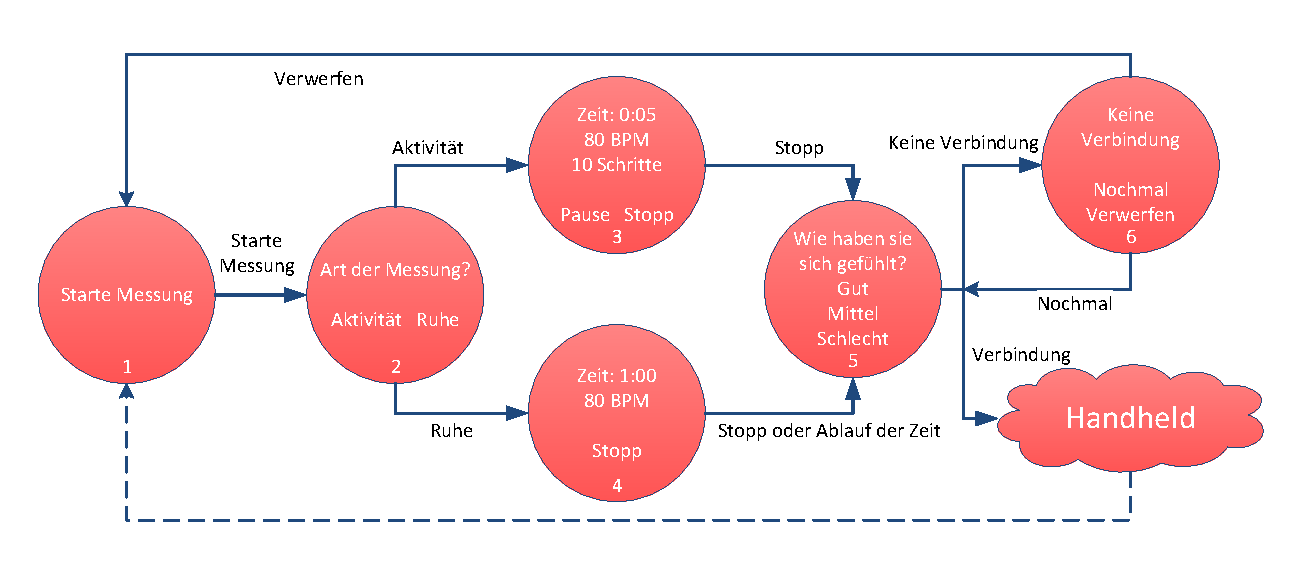
\includegraphics[scale=0.65]{images/structure_wearable.pdf}
	\caption{Struktur der Wearable-App}
	\label{fig:structure_wearable}
\end{figure}
\bigskip

Das Handheld-Gerät soll sich kontinuierlich in Bereitschaft zum Empfang von Messdaten befinden und diese verarbeiten können. Zusätzlich soll die App auf dem Handheld-Gerät über eine grafische Oberfläche zur Konfiguration und zur temporären Verwaltung von Messdaten verfügen. Ein Graph soll die Messungen übersichtlich visualisieren. Eine Bewertung der Daten ist an dieser Stelle nicht erforderlich.
\\[0.5cm] 
Das Handheld-Gerät soll die Messdaten per Bluetooth an ein Bluetooth-fähiges Endgerät weiter versenden können (z.B. PC oder Notebook). Es soll sowohl möglich sein, die Daten automatisch durch den Hintergrund-Dienst versenden zu lassen, als auch die Daten manuell über die grafische Oberfläche zu versenden. Die geplante Struktur der Handheld-App wird in Abbildung \ref{fig:strucure_handheld} dargestellt.

\bigskip
\begin{figure}[H]
	\visioToPDF{images/strucure_handheld.vsd}
	\centering
	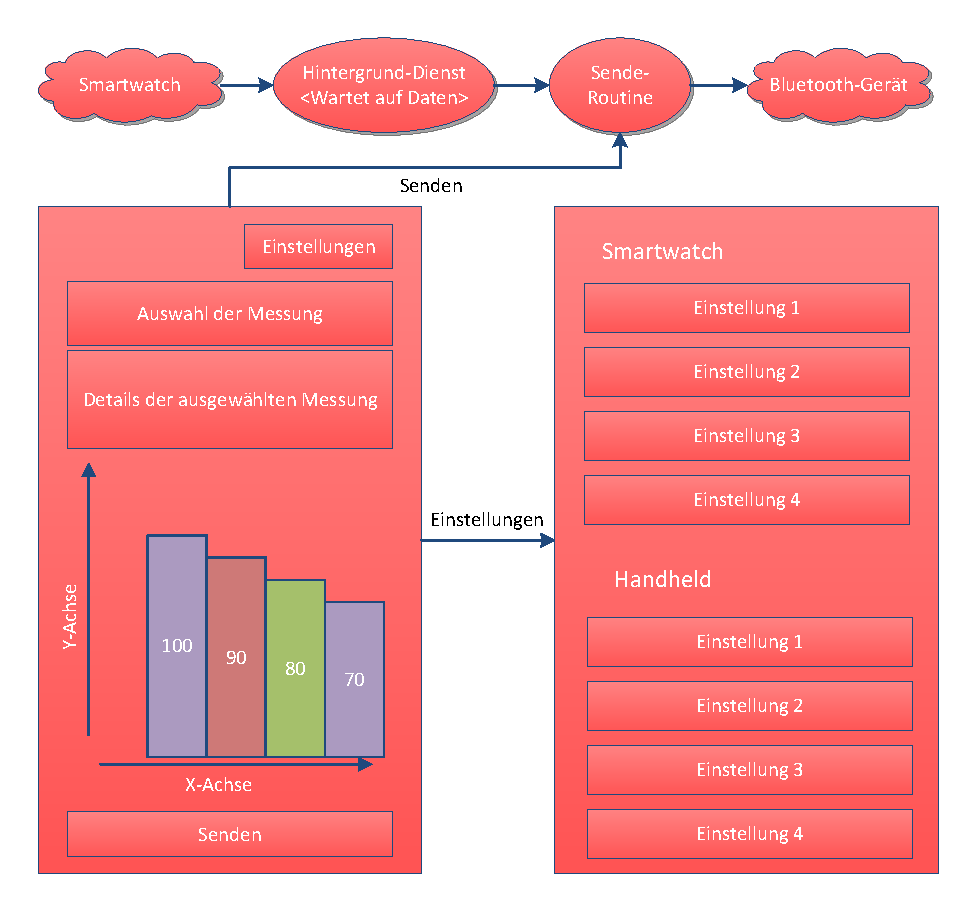
\includegraphics[scale=0.65]{images/strucure_handheld.pdf}
	\caption{Struktur der Handheld-App}
	\label{fig:strucure_handheld}
\end{figure}
\bigskip

\subsection{Vorbereitung}
Im Rahmen des Projektes werden eine Motorola Moto 360 Smartwatch und ein Samsung Galaxy S4 Smartphone als Testgeräte verwendet. Auf der Moto 360 läuft Android Wear in der Version 5.0 und auf dem Galaxy S4 läuft Android in der Version 4.4 (Cyanogenmod 11 Custom-Rom). Die Geräte sind grundsätzlich gekoppelt und die gleichnamige Google App "`Android Wear"' verwaltet auf dem Smartphone (im Hintergrund) die Verbindung zur Smartwatch. Die Entwicklung erfolgt mit Hilfe der Entwicklungsumgebung "`Android Studio"', die ebenfalls von Google veröffentlicht wurde. Dabei kann die Smartphone-App direkt über USB "`debugged"' werden, während der Debugging-Vorgang bei der Smartwatch über das gekoppelte Smartphone per Bluetooth gebrückt wird.

\subsection{Einschränkungen}
Bei Verwendung der Bluetooth-Library in der Qt-Framework Anwendung konnten Inkompatibilitäten nicht umgegangen werden (Näheres im Abschnitt QT Framework Anwendung). Aus diesem Grund soll die von der Handheld-App ausgehende Verbindung als TCP/IP Verbindung implementiert werden. Dabei soll ein UDP-Broadcast verwendet werden, um die Handheld-App im Netzwerk bekannt zu machen. Alternativ kann aber auch eine feste Adressierung angegeben werden. Da das Software-Paket sich letztlich an den gewöhnlichen Heimanwender richtet, ist grundsätzlich ein Heimnetzwerk mit Router und verbundenen Endgeräten zu erwarten und diese Anpassung sogar der Bluetooth-Variante vorzuziehen, da Bluetooth-Hardware zwar an Notebooks, jedoch vergleichsweise selten an feststehenden PCs verfügbar ist.

\subsection{Implementierung}
Die Implementierung teilt sich in drei Unterabschnitte zur Beschreibung: Die gemeinsame Bibliothek, die Wearable-App und die Handheld-App.
\subsubsection{Common-Library}
Die beiden Apps für das Wearable- und das Handheld-Gerät teilen sich eine Bibliothek um gemeinsame Datenstrukturen einfacher zu organisieren. \textit{HeartRateData} bildet einen Datensatz einer Messung ab, während \textit{HeartRateMeasure} eine umfassende Messung inklusive Modus, Stimmung und Durchschnittswert repräsentiert. Hier finden sich zusätzlich Methoden zur Übertragung und Konvertierung der Daten. So werden die Messdaten über die Android Wearable-Message-API als String im CSV-Format gesendet. Die statische Klasse \textit{HeartRateFile} bietet Methoden zum Laden und persistenten Speichern der genannten Datenstrukturen an. Diese Methoden werden nur auf dem Handheld-Gerät verwendet, jedoch könnte das Wearable-Gerät in einer möglichen Erweiterung auch eine persistente Speicherung der Daten vornehmen. In \textit{ByteCodes} werden Prefix-Byte-Codes für die serielle Übertragung per TCP angegeben. Der Empfänger der Daten muss dabei ebenfalls diese Byte-Codes kennen. In Abbildung \ref{fig:classes_common} werden diese Klassen dargestellt. Zusätzlich werden innerhalb der Common-Library alle verwendeten Grafiken zentral angelegt, um Redundanzen zu vermeiden.

\bigskip
\begin{figure}[H]
	\centering
	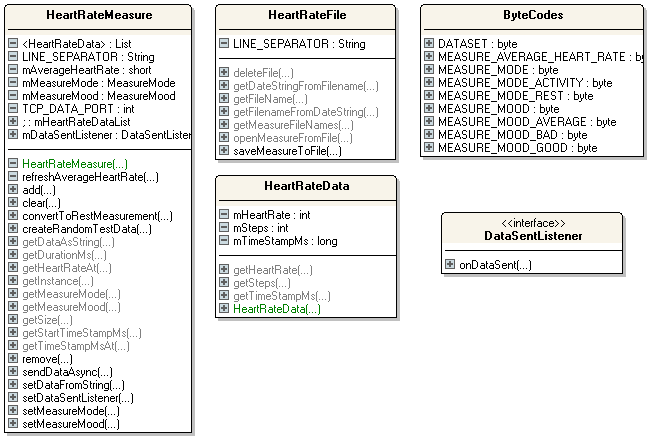
\includegraphics[scale=0.75]{images/classes_common.png}
	\caption{Klassendiagramm: Common-Library}
	\label{fig:classes_common}
\end{figure}
\bigskip

\subsubsection{Wearable-App}
Die Wearable-App teilt sich in verschiedene Grundkomponenten. Dabei bildet die Klasse \textit{WearActivity} das Zentrum der Ausführung. Sie wird von der Android-Klasse \textit{Activity} abgeleitet und dazu verwendet um eine Programmlogik mit Layout-Inhalten zu verknüpfen. Das WearActivity-Layout (siehe Abbildung \ref{fig:layout_wearactivity}) enthält alle grafischen Elemente, die zur Funktionalität benötigt werden:\\
\begin{minipage}[c]{0.5\textwidth}
	\begin{itemize}
		\item Zeitzähler inkl. Symbol
		\item Schrittzähler inkl. Symbol
		\item Puls
		\item Startbutton / Pausebutton
		\item Stoppbutton
		\item Hintergrundanimation
	\end{itemize}
\end{minipage}
\begin{minipage}[c]{0.5\textwidth}
	\begin{figure}[H]
		\centering
		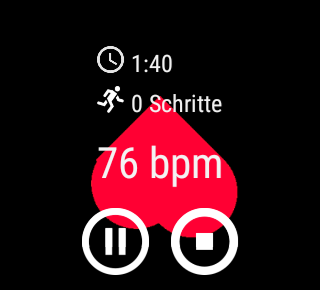
\includegraphics[scale=0.55]{images/layout_wearactivity.png}
		\caption{Layout: WearActivity}
		\label{fig:layout_wearactivity}
	\end{figure}
\end{minipage}
\\[0.7cm]
Die Hintergrundanimation (ein animiertes Herz-Symbol) besteht aus 32 Einzelbildern, die per XML-Animationsdatei aufeinander folgend abgespielt werden. Die Programmlogik der Hauptklasse \textit{WearActivity} basiert auf einem Zustandsautomaten. Elemente, die im jeweiligen Zustand nicht benötigt werden, werden ausgeblendet und umgekehrt. Analog zur Nummerierung in Abbildung \ref{fig:structure_wearable} finden sich die Zustände hier wieder. Die Zustände 2, 5 und 6 zur manuellen Abfrage von Informationen werden allerdings in externe Dialoge ausgelagert, da das Layout sich dort grundlegend ändert.
\\[0.5cm]
Diese Dialoge werden wiederum durch eigene Activitys repräsentiert und von der \textit{WearActivity} mittels Aufruf der Methode \textit{startActivity} gestartet. Sie liefern bei Beendigung einen entsprechenden Return-Wert. Abbildung \ref{fig:layout_dialogs} zeigt das Layout der drei Dialoge.
\bigskip
\begin{figure}[H]
	\centering
	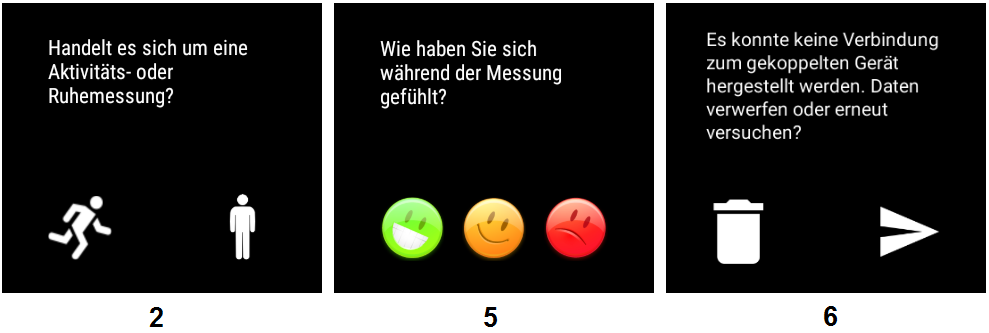
\includegraphics[scale=0.53]{images/layout_dialogs.png}
	\caption{Layout: Dialoge}
	\label{fig:layout_dialogs}
\end{figure}
\bigskip
Bei der Gestaltung der Wearable-Layouts wird das \textit{BoxInsetLayout} als Container verwendet, um eine äquivalente Darstellung auf quadratischen und runden Geräten zu erzielen und nur ein Layout für beide Display-Typen bereitstellen zu müssen. 
\\[0.5cm]
Abgesehen von den Activity-Klassen gibt es noch andere Klassen, die an der Umsetzung der Programmlogik innerhalb der Wearable-App beteiligt sind. So gibt es beispielsweise die Klasse \textit{RunningTimer}, die den Timer für Aktivitätsmessungen implementiert. Dabei kann eine beliebige Zeitspanne zum Auslösen des Events \textit{onTimerUpdate} angegeben werden. Das Event wird innerhalb der \textit{WearActivity}-Klasse genutzt um die Timer-Information auf der grafischen Oberfläche zu aktualisieren. Mit dem Event verbunden ist auch die regelmäßige Erinnerung (Vibrationsmuster bzw. Meldung), dass die App noch aktiv ist.
\\[0.5cm]
Daneben gibt es noch die Klasse \textit{RestTimer}, die die Ruhemessung unterstützt. Hier wird eine festgelegte Zeitspanne rückwärts gezählt und im Anschluss das Event \textit{onTimerFinished} ausgelöst. Analog zur Klasse \textit{RunningTimer} gibt es ebenfalls ein Event \textit{onTimerUpdate} zur Aktualisierung der Oberfläche.
\\[0.5cm]
Die wichtigste Komponente zur Erfassung der Sensor-Daten ist die Klasse \textit{SensorLogger}, die den Zugriff auf den Puls- und Schrittsensor verwaltet. Innerhalb des internen Events \textit{onSensorChanged} werden für beide Sensoren die entsprechenden Werte gespeichert und ein neues Event \textit{onSensorLog} zur Verwendung in der \textit{WearActivity}-Klasse abstrahiert. \textit{SensorLogger} bietet Methoden zum Starten, Stoppen und Pausieren des Logging-Vorgangs an. Auch das Messungsintervall kann festgelegt werden.
\\[0.5cm]
Eine weitere wichtige Komponente ist die Singleton-Klasse \textit{HeartRateDataSync}, die mit Hilfe der Wearable-Message-API einen String zu allen verbundenen Handheld-Geräten überträgt. Durch die Pfad-Angabe ("`/heartrate2go-message"') kann der Listener-Service am anderen Ende die App der Nachricht zuordnen.
\\[0.5cm]
Den letzten Bestandteil der Wearable-App bilden die Klassen \textit{DataLayerListenerService} und \textit{Settings}. Die Klasse \textit{DataLayerListenerService} wird von der Android-Klasse \textit{WearableListenerService} abgeleitet, die zur Verarbeitung eingehender Kommunikation seitens Wearable-API verwendet wird. Eine gleichnamige Klasse wird auf dem Handheld-Gerät ebenfalls verwendet, um die von \textit{HeartRateDataSync} ausgehenden Nachrichten zu empfangen. Auf dem Wearable-Gerät wird die Implementierung dieser Struktur lediglich für den Empfang von Settings-Werten benötigt. Dabei werden die Einstellungen innerhalb einer Hash-Map übertragen, da die Einstellungen selbst auch als Key-Value-Paare vorliegen. Die Klasse \textit{Settings} wird verwendet, um Zugriff auf die Klasse \textit{SharedPreferences} und die enthalten Einstellungen zu abstrahieren.
\\[0.5cm]
Die Zusammenhänge werden im Klassendiagramm der Abbildung \ref{fig:classes_wearable} noch einmal verdeutlicht.
\bigskip
\begin{figure}[H]
	\centering
	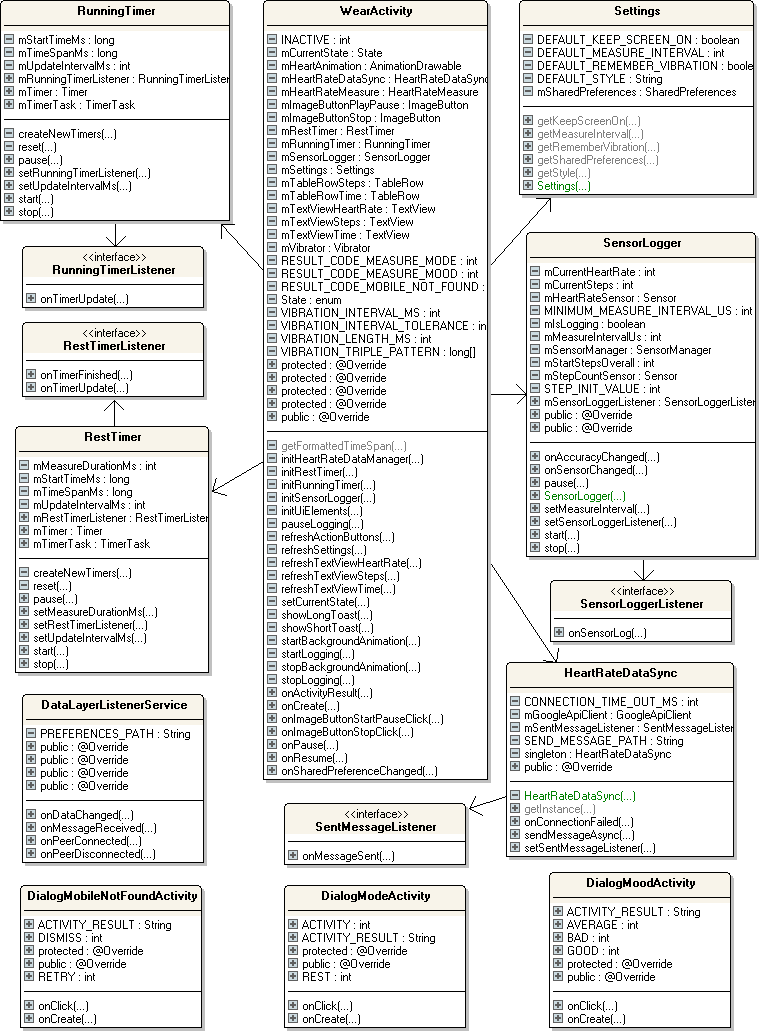
\includegraphics[scale=0.7]{images/classes_wearable.png}
	\caption{Klassendiagramm: Wearable-App}
	\label{fig:classes_wearable}
\end{figure}
\bigskip

\subsubsection{Handheld-App}
Die Handheld-App dient primär zur Weiterübertragung der über Bluetooth empfangenen Mess-Daten an eine externe Anwendung über TCP. Daneben werden auch Daten grafisch als Diagramm dargestellt und persistent vorrätig gehalten. Zur Diagramm-Darstellung wird sich der freien Library \textit{GraphView}\cite{graphview} bedient. Über eine Drop-Down-Liste kann eine Messung zur Anzeige ausgewählt werden. Eine ausgewählte Messung kann manuell über TCP versendet werden, gelöscht werden oder Beides gleichzeitig. Der Settings-Dialog der Handheld-App lässt verschiedene Einstellungen für Handheld-App und Wearable-App vornehmen, wie Abbildung \ref{fig:layout_settings} zeigt. Abbildung \ref{fig:classes_handheld} zeigt ein Klassendiagramm der Handheld-App.\\

\begin{minipage}[c]{0.5\textwidth}
	\begin{figure}[H]
		\centering
		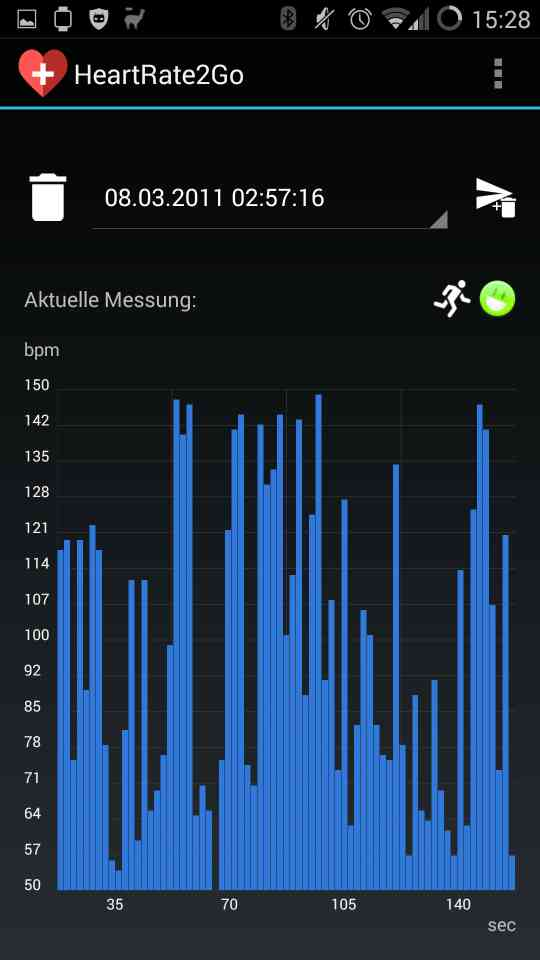
\includegraphics[scale=0.3]{images/layout_handheld.jpg}
		\caption{Layout: Handheld}
		\label{fig:layout_handheld}
	\end{figure}
\end{minipage}
\begin{minipage}[c]{0.5\textwidth}
	\begin{figure}[H]
		\centering
		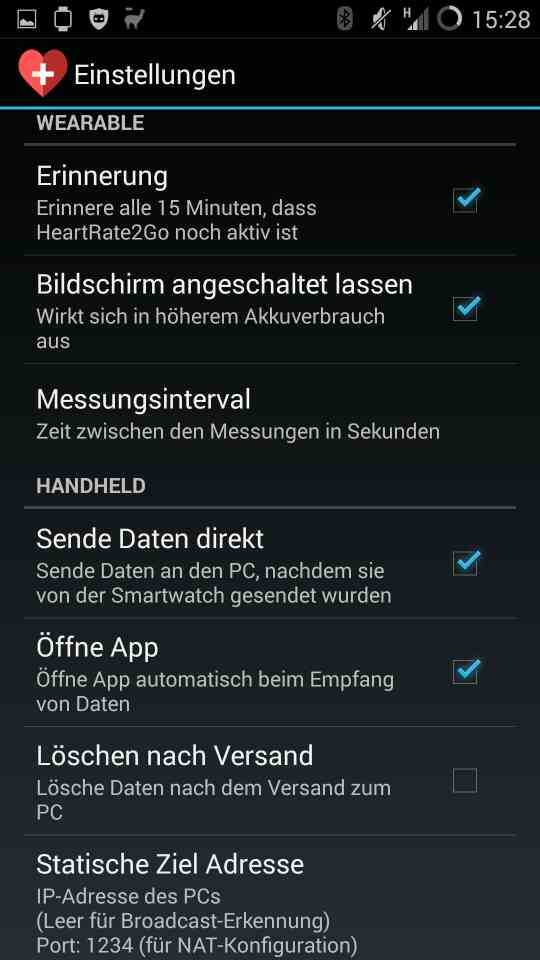
\includegraphics[scale=0.3]{images/layout_settings.jpg}
		\caption{Layout: Settings}
		\label{fig:layout_settings}
	\end{figure}
\end{minipage}
\\[0.7cm]

Die Handheld-App verfügt neben der Settings-Activity über eine Haupt-Activity \textit{HandheldActivity} zur Darstellung der Oberflächeninhalte. Die beschriebenen, überschaubaren Funktionen sind hier zentral verfügbar. Abbildung \ref{fig:layout_handheld} zeigt das zugehörige Layout.
\\[0.5cm]
Der Vorgang zum Senden der Messdaten über TCP ist innerhalb der Common-Klasse \textit{HeartRateMeasure} als Methode zu finden. Als Parameter muss lediglich die IP-Adresse übergeben werden. Innerhalb dieser Methode werden die Objektdaten mit Hilfe der Prefix-Byte-Codes serialisiert und als Byte-Stream versendet. Im Anschluss an den Sende-Vorgang berichtet das Event \textit{onDataSent} über den Status.
\\[0.5cm]
Die Klasse \textit{NetworkBroadcast} dient zur einfachen Identifizierung vor TCP-Gegenstellen im Netzwerk. Hierfür wird ein Magic-Packet per UDP-Broadcast in das lokale Netz gesendet und das Event \textit{onBroadcastFinished} ausgelöst, das bei Erfolg die IP-Adresse des Empfängers und dessen Antwort übergibt. Die Verwendung des Broadcasts ist einstellungsabhängig. Die Angabe einer statischen IP-Adresse ist ebenfalls möglich, womit der Broadcast umgangen wird.
\\[0.5cm]
Letztlich ist die Klasse \textit{DataLayerListenerService} für den Empfang der Messdaten von der Wearable-App verantwortlich und bildet das zentrale Element der Handheld-App. Bei eingehenden Messdaten wird der Service gestartet und sendet - je nach Einstellung - die Daten im Hintergrund unmittelbar zur TCP-Gegenstelle weiter. Entsprechend wird, bei aktivierter Einstellung zum Starten der App, die Oberflächen-Activity beim Empfangen von Daten mit gestartet und zeigt die aktuelle Messung an.
\\[0.5cm]


\bigskip
\begin{figure}[H]
	\centering
	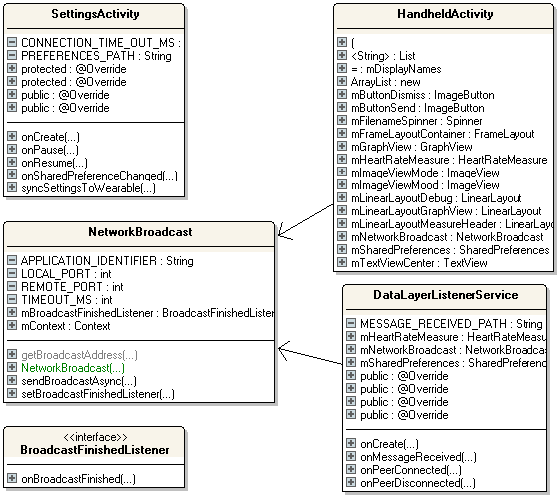
\includegraphics[scale=0.7]{images/classes_handheld.png}
	\caption{Klassendiagramm: Handheld-App}
	\label{fig:classes_handheld}
\end{figure}
\bigskip

\subsection{Evaluierung}
Es werden unterschiedliche Testfälle hinsichtlich Fehlerverhalten bei den vorgesehenen Ausführungsroutinen angefertigt und geprüft. Die Testfälle und deren Ergebnisse werden tabellarisch aufgelistet.
\subsubsection{Wearable-App}
Im Vordergrund steht bei der Wearable-App die ständige Definiertheit des Zustandsautomaten. In folgender Tabelle \ref{tbl:testcases_wearable} werden alle Zustände, Zustandsänderungen und Folgezustände aufgelistet und verifiziert. Die in Abbildung \ref{fig:structure_wearable} gezeigte Zustandsabfolge gilt hier als Referenz.

\begin{table*}[h]
	\centering
	  \rowcolors{1}{}{lightgray}
		\begin{tabularx}{\textwidth}{lXlc}
			\textbf{Zustand} 			& \textbf{Änderung} 	& \textbf{Folgezustand} 	&  \\
			Start (1) 						& Starte Messung 			& Messungsabfrage (2) 		& \ok \\
			Messungsabfrage (2) 	& Aktivität 					& Aktivitätsmessung (3) 	& \ok \\
			Aktivitätsmessung (3) & Pause 							& Aktivitätsmessung (3) 	& \ok \\
			Aktivitätsmessung (3) & Stopp 							& Stimmungsabfrage (5) 		& \ok \\
			Messungsabfrage (2) 	& Ruhe 								& Ruhemessung (4) 				& \ok \\
			Ruhemessung (4) 			& Stopp 							& Stimmungsabfrage (5) 		& \ok \\
			Stimmungsabfrage (5) 	& + Verbindung 				& Start (1) 							& \ok \\
			Stimmungsabfrage (5) 	& - Verbindung 				& Retry-Abfrage (6) 			& \ok \\
			Retry-Abfrage (6) 		& Retry + Verbindung 	& Start (1) 							& \ok \\
			Retry-Abfrage (6) 		& Retry - Verbindung 	& Retry-Abfrage (6) 			& \ok \\
		\end{tabularx}
		\caption{Testfälle: Wearable}
		\label{tbl:testcases_wearable}
\end{table*}

\subsubsection{Handheld-App}
Die Handheld-App muss in der Rolle des Daten-Vermittlers zwischen Wearable-Gerät und IP-Endgerät die Messdaten zuverlässig und unverändert weiterleiten. Die korrekte Darstellung von Messdaten ist ebenfalls ein Testkriterium. Außerdem wird die Anwendung und Übertragung von Einstellungen geprüft. Die nachstehende Tabellen \ref{tbl:testcases_handheld_behavior} und \ref{tbl:testcases_handheld_settings} zeigen die Testkriterien auf.

\begin{table*}[h]
	\centering
	  \rowcolors{1}{}{lightgray}
		\begin{tabularx}{\linewidth}{Xc}
			\textbf{Testfall}																		& \\
			Daten auf grafischer Oberfläche korrekt anzeigen		& \ok \\
			Daten mit Hintergrund-Dienst versenden							& \ok \\
			Daten mit grafischer Oberfläche versenden						& \ok \\
			Toast über Versende-Status anzeigen									& \ok \\
			Daten löschen			 																	& \ok \\
			Zufällige Daten erzeugen (Debugmodus)								& \ok \\
			Alle Datensätze versenden (Debugmodus)							& \ok \\
			Daten bei nur bei erfolgreicher Verbindung löschen	& \ok \\
		\end{tabularx}
		\caption{Testfälle: Handheld-Verhalten}
		\label{tbl:testcases_handheld_behavior}
\end{table*}

\begin{table*}[h]
	\centering
	  \rowcolors{1}{}{lightgray}
		\begin{tabularx}{\linewidth}{Xlc}
			\textbf{Einstellung}						& \textbf{Typ} 				& \\
			Erinnerung											& Wearable 						& \ok \\
			Bildschirm angeschaltet lassen 	& Wearable 						& \ok \\
			Messungsintervall 							& Wearable 						& \ok \\
			Sende Daten direkt 							& Handheld 						& \ok \\
			Öffne App automatisch						& Handheld 						& \ok \\
			Löschen nach Versand						& Handheld 						& \ok \\
			Statische Ziel-Adresse					& Handheld 						& \ok \\
			Debug-Modus							 				& Handheld 						& \ok \\
		\end{tabularx}
		\caption{Testfälle: Handheld-Einstellungen}
		\label{tbl:testcases_handheld_settings}
\end{table*}

%\lstset{language=Java}
%\begin{lstlisting}[caption=Listing, label=lst:Listing]
%\end{lstlisting}

%\begin{shaded}
%Text in Textbox
%\end{shaded}

%\ref{sec:hauptteil}
%\cite{audio_architecture}
\newpage
\section{Qt-Framework Anwendung}

\subsection{Model-View Konzept}

In der Praxis werden viele User Interfaces mit dem MVC Pattern realisiert. Dieses Pattern besteht aus der View, dem Controller und dem Model. In diesem Zusammenhang wird eine strikte Trennung der einzelnen Schichten angestrebt. Das Ziel dieses Ansatzes, liegt in dem Austausch der View, ohne eine Anpassung der internen Datenstruktur durchführen zu müssen. Eine weitere Variante dieses Konzeptes ist das Model/View Konzept. Hierbei wird die View mit dem Controller kombiniert. Die Aufgabe der View es ist mit Hilfe des Models dem Benutzer die Informationen anzuzeigen. Der Controller reagiert lediglich auf Interaktion des Benutzers mit der View. Zusätzlich kann bei einer Model/View Architektur das Konzept eines „delegates“ eingeführt werden. Dieser besitzt die Aufgabe, die einzelnen Datenelemente des Models benutzerspezifisch anzuzeigen oder auf bestimmte Veränderungen des Datenbestandes von Seiten des Benutzers auf der View zu reagieren. Das Zusammenspiel der einzelnen Komponenten wird in Abbildung 1 nochmals graphisch veranschaulicht. \\

\begin{center}
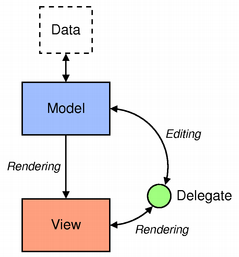
\includegraphics[scale=1.0]{images/ModelView.png}  \\
\end{center}

In Abbildung 1 wird deutlich, dass eine Trennung zwischen der Speicherung und der Darstellung der Daten besteht. Die Aufgabe des Models besteht darin, der View und dem Delegate minimalistische Schnittstellen für die Kommunikation bereitzustellen. Die Kommunikation zwischen den einzelnen Komponenten wird in QT mit Hilfe des Signal und Slot Konzeptes realisiert. Findet eine Änderung am Datenbestand des Models statt, wird ein Signal an die View und den entsprechenden Delegate geschickt. Diese rufen die entsprechenden Slots auf und aktualisieren die View. Im umgekehrten Fall, wenn der Benutzer die Daten via View verändert, schickt diese ein Signal an das Model und den Delegate. Ein weiteres Hilfsmittel der View ist der Modelindex. Dieser Index wird verwendet, um die einzelnen Informationen aus dem Datenbestand zu lesen. \\

Ein Modelindex ist eine Referenz auf einen einzelnen Datensatz des Models. Durch die Zuhilfenahme eines Delegates, kann dieser benutzerspezifisch auf der View dargestellt werden. Diesbezüglich muss erwähnt werden, dass es mehrere Möglichkeiten für die Erstellung der View unter QT existieren. Eine Möglichkeit ist die Erstellung mittels QT Widgets. Diese können durch Qt bereitgestellte Klassen erzeugt werden. Hierbei ist eine eindeutige Trennung zwischen View und Model schwer möglich. Eine andere Variante ist die Erstellung mittels QML. QML ist eine Art Beschreibungssprache für Benutzeroberflächen. Hierbei muss lediglich eine Beschreibung der GUI angegeben werden. Diese ist so allgemein gehalten, dass Designer oder UI-Entwickler ohne irgendwelche Vorkenntnisse einer Programmiersprache eine View anfertigen können. Der Vorteil hiervon liegt in der klaren Trennung der einzelnen Aufgaben. Ein Designer kann sich ausschließlich um das UI kümmern und ein Software-Entwickler um das dazugehörige Model und den Controller. Diesbezüglich existiert eine klare Trennung zwischen dem Model und der View.\\

In Qt sind alle Model Klassen von der Abstrakten Basisklasse QAbstractItemModel abgeleitet. Diese Basisklasse bietet eine Vielzahl an Schnittstellen für die Kommunikationen mit der View an. Um auf eine gegeben Datenstruktur besser reagieren zu können, bietet QT 3 besondere Model-Typen an. Diese Modeltypen sind: QListModel, QTableModel und QTreeModel. Mit Hilfe dieser 3 Modeltypen, kann eine Vielzahl der Anwendungsbereiche abgedeckt werden. In diesem Projekt ist ausschließlich ein QAbstractListModel verwendet worden. Zur Umsetzung des Model View/Konzeptes wurde für die Bereitstellung der UI die Beschreibungssprache QML verwendet. Für die Implementierung des Models wurde die bereits von Qt bereitgestellte Klasse QAbstractListModel verwendet. Hierbei ist eine neue Unterklasse von QAbstractListModel erzeugt und die entsprechenden Methoden für die Kommunikation mit der View neu implementiert worden. Als Datenstruktur wurde eine QList mit entsprechenden Datenobjekten gewählt. Die Datenobjekte besitzen die Aufgabe, die einzelnen Messwerte einer Messung zu kapseln. Eine Vielzahl der QML Elemente wie beispielsweise eine ListView oder TableView bieten standartmäßig eine Property „model“ an, welche die Verknüpfung mit dem entsprechenden Model realisiert. Des Weiteren kann mittels QML ein delegate Objekt erzeugt werden. Mit dessen Hilfe, können beispielsweise die Einträge in einer ListView bestmöglich auf die Wünsche des End-Benutzers angepasst werden. \\

Der Vorteil des QT Frameworks ist die automatische Anpassung der GUI an eine Änderung des internen Datenbestandes. Der Entwickler muss lediglich dem Model mitteilen, wann eine Änderung am Datenbestand des Models durchgeführt wurde. Infolgedessen übernimmt das Framework die komplette Aktualisierung der GUI. Der umgekehrte Fall, dass der Benutzer die Daten mittels GUI verändern kann, ist im Projektverlauf nicht implementiert worden. \\

Für die bestmögliche Darstellung der gesammelten Daten, mussten mehrere Diagramme erstellt werden. Hierbei bestand die Möglichkeit, alle Diagramme über die von QT bereitgestellten Klassen zu erzeugen, oder ein bereits vorhandenes auf QT basierendes Modul namens QCustomPlot zu verwenden. Dieses Modul kapselt die von QT bereitgestellten „Paint“ Klassen und gibt dem Benutzer eine Vielzahl an bereits vorimplementierten Diagramm-Typen. Ursprünglich wurde diese Third-Party Modul für den Einsatz mit QT Widgets konzipiert. Diesbezüglich musste eine Portierung in QML durchgeführt werden. Folglich konnten einige Funktionalitäten wie beispielsweise das Zoomen nicht in QML überführt werden. Die Portierung ist mittels der QCustomPlot Support Seite durchgeführt worden. \\

TODO: Quellen einfügen
Quellen:

http://qt-project.org/doc/qt-4.8/modelview.html

http://qt-project.org/doc/qt-4.8/model-view-programming.html

http://sysmagazine.com/posts/181712/

http://doc.qt.io/qt-5/qtqml-cppintegration-interactqmlfromcpp.html

http://qt-project.org/doc/qt-4.8/qmlevents.html

http://qt-project.org/doc/qt-4.8/qtbinding.html\#exchanging-data-between-qml-and-c

http://www.qcustomplot.com/index.php/support/forum/172

http://www.qcustomplot.com/index.php/tutorials/settingup

The Book of QT 4.0 Daniel Molkentin


\subsection{Umsetzung mittels QML}

\subsection{Datenübertragung}
\subsubsection{TCP-Server}
Die Qt-Komponente der HeartRate2Go Anwendung agiert für die Datenübertragung als TCP-Server. Die Umsetzung wird mit Hilfe der QTcpServer-Klasse der Qt-Bibliothek vorgenommen\cite{qtcpserver}. Eingehende Verbindungen werden in der TcpConnection-Klasse verarbeitet, die sich von der QThread-Klasse ableitet und dadurch die asynchrone Verarbeitung mehrerer Verbindungen sicherstellt.\\
\\
Wenn der TcpServer eine eingehende Verbindung annimmt, erzeugt er ein Objekt der TcpConnection-Klasse und übergibt ihr den Connection-Socket. Anschließend erhält der Thread des TcpConnection-Objekts die Kontrolle über diese Verbindung.\\
\\
Die Thread-Loop der TcpConnection-Klasse wartet auf eingehende Bytes und hängt diese an ein QByteArray-Objekt an. Nach dem Trennen der Verbindung wird dieses QByteArray zur weiteren Auswertung an den DataReceiver übergeben.

\subsubsection{Server-Discovery}
Um bei der Verwendung einer TCP/IP-Datenübertragung eine sichere Konnektivität zwischen Smartphone und Desktop-PC zu gewährleisten, muss der Anwender einen zusätzlichen Konfigurationsaufwand zur Ermittlung und Konfiguration der IP-Adresse in Kauf nehmen. Die HeartRate2Go Desktop-Anwendung verfügt deshalb über einen UDP-Server, der mittels eines einfachen Broadcast-Protokolls die Server-Discovery automatisiert und so dem Anwender den Konfigurationsaufwand gänzlich erspart\footnote{Für Netze in denen Broadcast-Messages blockiert, oder über Netz-Grenzen hinweg geroutet werden, ist weiterhin eine manuelle Konfiguration notwendig.}.\\
\\
Die Implementierung des UDP-Servers in der BroadcastReceiver-Klasse erfolgt durch Ableitung von QThread und einem auf Port 45454 gebundenen QUdpSocket-Objekt\cite{qudpsocket}. Die Thread-Loop wartet anschließend auf eingehende Datagramme.\\
\\
Beim Eintreffen eines Datagramms wird zunächst überprüft, ob es sich dabei um das erwartete Magic-Packet handelt. Ist dies der Fall, wird das Datagramm an den Absender an Port 45455 zurück gesendet. Der ursprüngliche Absender kann dadurch beim Empfang der Antwort die IP-Adresse des Servers ermitteln und eine TCP-Verbindung herstellen. Hat sich das Magic-Packet als falsch herausgestellt, wird das Datagramm verworfen.\\
\\
Bei dem Magic-Packet handelt es sich um den ASCII-String der UUID ''86417ce4-4f19-4a59-ae27-f404653e9751''.

\subsubsection{DataReceiver}
Die DataReceiver-Klasse nimmt das eigentliche Parsing des vom Smartphone erhaltenen Byte-Vektors unter Beachtung der Network-Byte-Order vor. Sie abstrahiert lediglich die Byte-Vektor-Darstellung der Daten von der vom Modell benötigten Listen-Repräsentation. Die Klasse ist als Singleton implementiert, da sie aufgrund des verwendeten Signal-Slot-Konzepts instanziiert werden muss.\\
\\
Der Parsevorgang wird mit Hilfe eines Zustandsautomaten realisiert, da die zu erwartenden Daten einem festgelegten Schema folgen müssen.\\
\\
Nach einem erfolgreichen Parsevorgang werden die so gewonnenen Datensätze an die ImportExport-Klasse übermittelt und der FilterController mit einem Signal über das Eintreffen neuer Daten benachrichtigt.\\
\\
In den Tabellen \ref{tbl:pdu} und \ref{tbl:datafield-description} wird das für die Datenübertragung verwendete Protokoll erläutert. Das \textit{Data}-Datenfeld darf dabei als einziges Datenfeld mehrfach vorkommen und dient zur Übertragung der einzelnen vorgenommenen Messungen während eines Gesamt-Messvorgangs. Bei einer Ruhemessung ist hier ein einziger Datensatz zu erwarten. Bei einer Aktivitätsmessung ist die Anzahl der \textit{Data}-Datensätze abhängig von der Dauer der Messung und des konfigurierten Messintervalls. Weiterhin dient ein leeres \textit{Data}-Feld als Sentinel um das korrekte Ende der Übertragung (EOT) zu signalisieren.
\begin{table*}[h]
	\centering
		\begin{tabularx}{\textwidth}{l|l|l|X}
			\hline
			Bezeichnung & Byte & Länge & Beschreibung \\
			\hline
			\hline
			Mode & \texttt{0x00} & 1 & Typ der Messung\\
			\hline
			Mood & \texttt{0x01} & 1 & Gemütszustand bei der Messung\\
			\hline
			Average & \texttt{0x02} & 2 & Durchschnitt aller Messwerte\\
			\hline
			Data & \texttt{0xff} & 12/0 & Datensatz eines Messpunktes/EOT\\
			\hline
		\end{tabularx}
		\caption{Protokoll-Datenfelder der Datenübertragung (Länge in Byte)}
		\label{tbl:pdu}
\end{table*}

\begin{table*}[h]
	\centering
		\begin{tabularx}{\textwidth}{l|l|l|X}
			\hline
			Bezeichnung & Länge & Typ & Beschreibung \\
			\hline
			\hline
			Zeitstempel & 8 & ulong & Zeitpunkt in Millisekunden des aktuellen Messpunktes\\
			\hline
			Puls & 2 & ushort & Pulswert dieses Messpunktes\\
			\hline
			Schritte & 2 & ushort & Anzahl der Schritte (inkrementell)\\
			\hline
		\end{tabularx}
		\caption{Aufbau des \textit{Data}-Datenfeldes aus Tabelle \ref{tbl:pdu}}
		\label{tbl:datafield-description}
\end{table*}

\subsection{Datenhaltung}
\subsubsection{SQLite}
Zur Speicherung sämtlicher Messungen, und damit verbundenen Datensätze, wird auf die SQLite-Datenbankengine zurückgegriffen. Das Qt-Framework bietet mit der QSqlDatabase-Klasse eine Abstraktion zu vielen SQL-basierenden Datenbankengines an\cite{qsqldatabase}. Unter anderem unterstützt sie SQLite. Der Datenbank-Container wird plattformunabhängig im Benutzerverzeichnis des die Anwendung ausführenden Benutzers im Verzeichnis ''HeartRate'' gespeichert.

\subsubsection{Datenbankschema}
\begin{figure}[H]
	\centering
	\visioToPDF{images/database-schema.pdf}
	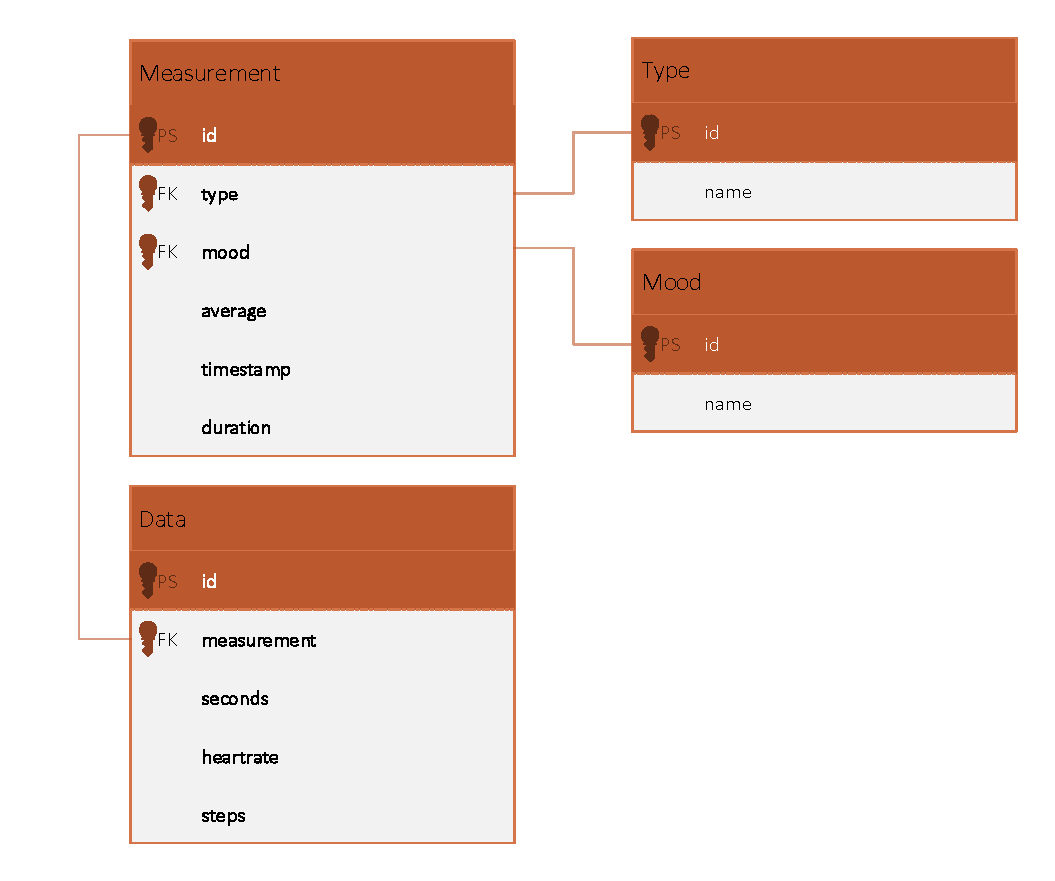
\includegraphics[width=0.9\textwidth]{images/database-schema.pdf}
	\caption{Das SQLite Datenbankschema}
	\label{pic:database-scheme}
\end{figure}

\begin{table*}[h]
	\centering
		\begin{tabularx}{\textwidth}{l|X}
			\hline
			DB-Tabelle & Beschreibung \\
			\hline
			\hline
			Measurement & Speichert allgemeine Informationen \textbf{einer} Messung\\
			\hline
			Data & Speichert die einzelnen Messwerte zu einem \textit{Measurement}-Eintrag\\
			\hline
			Mood & Speichert die möglichen Gefühlszustände, die jeder Messung zugeordnet werden\\
			\hline
			Type & Speichert die möglichen Messungstypen, die jeder Messung zugeordnet werden\\
			\hline
		\end{tabularx}
\end{table*}




\newpage
\section{Fazit}
% muss rein (von Conrad):
% implementierte Anwendung und deren Funktionalitäten
% Verwendete Frameworks mit Begründung
% Beschreibung des Software-Designs
% Beschreibung des User Interfaces
% kurze Beschreibung der Bedienung der Anwendung
% weitere sinnvolle Angaben
% Verwendete Literatur und Quellen
\subsection{Retrospektive} \label{sec:Retrospektive}

% Retrospektive (kritischer Rückblick, Vergleich zu ursprüngliche Planung)
% - Schwierigkeit bei der Entscheidung, was schaffen wir in der vorgegen Zeit?
% - Übertragung von Smartphone zur GUI nicht über Bluetooth möglich 
% - Print Dialog
% Ausblick (Wie kann das Projekt weiter entwickelt werden)
\subsection{Ausblick} \label{sec:Ausblick}
Wie schon im Konzeptpapier erwähnt, besteht die Möglichkeit, das Projekt \textit{HeartRate2Go} zu publizieren und es so anderen Anwendern zugänglich zu machen. Hierzu könnte es durch weitere Funktionen erweitert werden. Einige dieser Anwendungen finden sich schon im Konzeptpapier unter 2.b. Optionale Funktionen, zum Beispiel: das Anlegen von Benutzerprofilen. \\ Dies geschieht derzeit nur ansatzweise, die gesendeten Werte werden für jedes Benutzerprofil des Betriebssystems separat abgespeichert. Jedoch ist eine Anamneseabfrage noch nicht möglich. In dieser würde nach Alter, Geschlecht, Größe, Gewicht, maximaler und minimaler Pulswert für die beiden Messwerttypen gefragt werden. So wäre auch eine erste Einschätzung der gemessenen Werte möglich.
\\
Ein anderer Punkt, ist die Berechnung des Kalorienverbrauchs. Zwar wird während einer Aktivitätsmessung die Anzahl der Schritte angezeigt, jedoch war es leider in der vorgegeben Zeit nicht möglich, der dadurch resultierende Kalorienverbrauch zu errechnen. Hierfür ist auch die Schrittlänge nötig, die mit einem Benutzerprofil einhergeht. \\
Des Weiteren stand zur Diskussion, ob dem Nutzer die Möglichkeit gegeben werden soll, Marker zusetzen, die eine besondere Situation kennzeichnen und in der späteren Ansicht speziell angezeigt werden. Dies ist bei einer, vom Hausarzt angeordneten, Langzeit-EKG-Messung ein wichtiger Teil, auch für die spätere Bewertung der Messung. \\
Da das \textit{HeartRate2Go-Programm} auf allen Betriebssysteme läuft, wäre eine App für das iOS-Betriebssystem auch praktisch. Der Zeit existiert die \textit{HeartRate2Go-App} nur für Android. Die Erstellung einer iOS-App war jedoch leider nicht möglich, da hierfür keine passende Apple-Komponenten zur Verfügung standen.\\
Die Umsetzung der genannten Punkte scheiterte an der begrenzten Zeit, die für dieses Projekt zur Verfügung stand. \\
% - Messung per Smartphone
% - siehe Konzeptpaper (fehlende Nice-to-have Lasten)
% 	- Benutzerprofile anlegen und abspeichern mit Anamneseabfrage
% 	- Berechnung des Kalorienverbrauchs
% - Marker setzten
% - iOS-App

% Drucken und mit abgeben:
% Ausgabe der Projektarbeit und Nutzungsvereinbarung
% Ehrenwörtliche Erklärung

\newpage

%% Literaturverzeichnis
%% ==> Eine Datei 'literatur.bib' wird hierf�r ben�tigt.
%% ==> Sie m�ssen hierf�r BibTeX verwenden (Projekt | Eigenschaften... | BibTeX)

\addcontentsline{toc}{section}{Literaturverzeichnis}
%\nocite{*} %Auch nicht-zitierte BibTeX-Eintr�ge werden angezeigt.
%\bibliographystyle{alpha} %Art der Ausgabe: plain / apalike / amsalpha / ...
%\bibliography{literatur} %Eine Datei 'literatur.bib' wird hierf�r ben�tigt.

\def\bibfont{\footnotesize}
\printbibliography[title={Literaturverzeichnis}]

%% Abbildungsverzeichnis
%\clearpage
%\addcontentsline{toc}{section}{Abbildungsverzeichnis}
%\listoffigures

%% Tabellenverzeichnis
%\clearpage
%\addcontentsline{toc}{section}{Tabellenverzeichnis}
%\listoftables


%%%%%%%%%%%%%%%%%%%%%%%%%%%%%%%%%%%%%%%%%%%%%%%%%%%%%%%%%%%%%
%% ANH�NGE
%%%%%%%%%%%%%%%%%%%%%%%%%%%%%%%%%%%%%%%%%%%%%%%%%%%%%%%%%%%%%
\appendix
%% ==> Schreiben Sie hier Ihren Text oder f�gen Sie externe Dateien ein.

%\input{Dateiname} %Eine Datei 'Dateiname.tex' wird hierf�r ben�tigt.

\end{document}

